\chapter{Introduction}
\label{cha:intro}

Today, data is produced at an overwhelming rate
that cannot be processed by traditional methods.
For example, Cisco has estimated in its annual white paper
that data produced by people, machines, and things
is around 500 zettabytes, in contrast to a much smaller volume
of data that can be feasibly stored~\cite{index2018forecast}.
Researchers and industry practice have accordingly recognized the demand
for a new paradigm of computing where data is
distributed (processed in parallel over many devices),
transient (processed as it arrives and discarded),
and temporally structured (considered with respect to time).
This \emph{stream processing} paradigm has given rise to an increasing number
of modern data processing software frameworks.\footnote{
  E.g.: Kinesis from Amazon~\cite{AmazonKinesis}, Timely~\cite{Timely} and Differential Dataflow~\cite{mcsherry2013differential} from Materialize, and Spark~\cite{SparkStreaming}, Storm~\cite{Storm}, and Flink~\cite{Flink} from the Apache Software Foundation.
  See \Cref{cha:background,cha:rw}.
}
Broadly construed, the stream processing paradigm is exemplified not only by these dedicated frameworks, but also by many other modern systems: these include microservices deployed in the cloud; IoT and other edge devices, which operate in response
to sensor data~\cite{shi2016edge, ashton2009internet}; and programmable network switches,
which can be used to push some of this expensive streaming computation
into the network.
Stream processing also has theoretical justification in the \emph{streaming model of computation},
where items arrive one at a time and are processed as they arrive, ideally using
a minimal amount of space and time per element.
In this thesis, we reconsider the stream processing paradigm through the lens of \emph{programming languages}, by investigating software abstractions which are type-safe, deterministic, and performant: that is, which save programmers from common mistakes and ensure that the deployed program meets their intent.

\section{Motivation}

Although research in stream processing can be traced back two decades from within the database community~\cite{Aurora,Borealis,STREAM2004,Telegraph,ABW2006CQL},
and even earlier in programming languages and compilers~\cite{burge1975stream,stephens1997survey,thies2002streamit},
researchers have devoted inadequate attention to software correctness (see our short paper~\citeMain{stanford2022correctness}).
Today's systems are difficult to test for correctness and debug. In the context of Apache Spark, researchers found that bugs are time-consuming to diagnose due to a number of issues related to distributed deployment (e.g., a bug only shows up on a particular input item out of millions, in a particular distributed execution, or in the presence of faults)~\cite{gulzar2016bigdebug}. For streaming applications in Apache Flink, user studies have demonstrated that the state of practice is limited to unit and integration testing~\cite{vianna2019exploratory}.
For some use cases, building and deploying a correct application in today's systems can require either significant expertise in distributed systems or a good deal of experience with developing and debugging for the specific streaming framework in question. We posit that there is therefore both a need and a research opportunity for more sophisticated testing and formal correctness techniques. With the right abstractions and automated formal tools, programming correct distributed applications over data streams could be much easier for inexperienced users than it is today.

From a programming languages viewpoint, two problems stand out in particular. First, existing systems lack \emph{safe semantics}. We will elaborate on what we mean by safety when describing our proposed model; in brief, existing systems lack \emph{fine-grained type safety} with respect to differences in streams and how they are parallelized, and lack \emph{determinism} with respect to all possible parallel or distributed executions. The requirement for determinism has been articulated since the early history of streaming (see~\cite{stonebraker20058}, requirement 4) but remains absent in practice.

Second, existing systems disagree on basic details about how streams are parallelized. Points of disagreement include, but are not limited to: are stream items ordered or unordered? Are streams parallelized explicitly (via syntax) or implicitly (by the system)? Can parallel instances of a stream operator communicate via external state or communicate with external services? Can parallel instances communicate with each other, through mechanisms such as broadcasting a message to all other instances? We will discuss some of these differences in more detail in \Cref{cha:background}. In summary, \emph{there is no common, agreed-upon semantics for stream processing.} The lack of a common language and semantics makes it difficult to design formal tool support, especially if we want the ideas to be applicable across systems.
% Zack: are you arguing you have an all-encompassing language?
% Answer: not necessarily, but this is hopefully progress towards that.
% Hopefully this becomes clearer later in the text.

Besides semantic bugs, misunderstanding the details of parallelism in the system is also an easy way to overlook performance bottlenecks. Performance is critical for stream processing systems, but is not formally guaranteed (see e.g.,~\cite{lopez2016performance,dias2018dsp-survey,hoffmann2018snailtrail,bordin2020dspbench}); it can be less predictable and reliable than performance at the level of hardware or operating systems.

Semantic language-level issues certainly do not constitute the only barriers to software development in today's stream processing systems. Many other user-facing problems are of critical importance -- to name a few, debugging tool support, boilerplate code and configuration, input and output, and interfacing with the operating system and with other services. We do not focus on these problems in this thesis. However, from personal experience programming in stream processing frameworks, we believe that the semantic language-level issues we focus on do have a significant programming impact.

\section{A Programming Example: Values and Barriers}
\label{ex:value-barrier}

To further motivate our approach, consider the following concrete minimal example.
Three streams arrive in the system: two parallel streams of \emph{values}, which are integers (\texttt{int}), and a stream of \emph{barriers}, which are of the unit type (\texttt{unit}).
All of these events are timestamped when they arrive.
The values are parallel in the sense that they arrive in the system in parallel at multiple nodes (in this case two, for simplicity).
The barriers all arrive in one stream at a single node.
Our task is to output the ``sum of the values occurring between every two adjacent barriers.'' That is, whenever a barrier occurs, we want to output the sum of all the values with timestamp values since the previous barrier. This computation is sometimes known as an \emph{event-based window} because the window of events to aggregate depends on the occurrence of certain events (in this case, the occurrence of a barrier)~\cite{EventBasedWindow}.
We assume in this scenario that barriers are much less frequent than values, and not parallelizable; i.e. they require global synchronization across all nodes.

It turns out that such a parallel computation is rather subtle to program in existing systems. High-level query libraries (e.g., based on SQL) typically don't provide event-based windows directly but require deriving them from expensive joins.
\Naive{}ly, one way to solve the problem is to send all the values to the same node as the barrier, but this results in a central bottleneck and does not exploit any parallelism.
To solve the problem, one solution is to \emph{broadcast} the barrier stream to all other parallel nodes; the broadcast primitive is provided in a few systems such as Flink and Timely Dataflow~\cite{BroadcastStateFlink,BroadcastStateTimely}.
Once the stream is visible from all parallel nodes, each of those streams then has to solve only a local windowing problem.
The local event-based window can be achieved in multiple ways, depending on the system; at the core, it requires a re-timestamping operation to
group value events with respect to the barrier-window that they fall into,
where the window is either identified by a number in sequence (1 for the first window, 2 for the second, and so on) or by the timestamp of the barrier it corresponds to.
After values are timestamped appropriately, they can be added by-timestamp (a built-in operation in all systems) and then aggregated across parallel nodes (also standard) for the final output at each barrier.

The value-barrier example is simple, but emblematic of the broader problem: when parallel structure is not simply embarrassingly-parallel and requires some synchronization (in this case, synchronization based on the barrier stream), embarrassingly-parallel abstractions fail.
We claim that there is a better way; that parallelism can be expressed in a semantically meaningful manner at a higher-level of abstraction.
Going back to the features that we want to provide in existing systems:
\begin{itemize}
  \item \emph{Fine-grained type safety:} Fundamentally, the value stream and the barrier stream are quite different. The barrier stream arrives only at one node; the value stream arrives in parallel at many nodes. But some existing systems do not distinguish between these two kinds of streams at the typing level. So operations that interact between sequential streams and parallel streams are not type-safe: a consumer expecting a sequential stream may get a parallel one at many nodes resulting in a software bug.
  \item \emph{Determinism:} In the ``correct'' computation, the output value at each barrier is a deterministic function of the inputs (including their timestamps). In our experience it is very easy to write this computation incorrectly and accidentally window values in a nondeterministic manner, e.g., if events are grouped as-they-arrive instead of by timestamp. Yet the only way to detect this sort of nondeterminism is to run the system and hope that an execution appears where the events arrive in a different order than the timestamps indicate, which is highly unlikely when the rate of events is sparse and only becomes likely under heavy input load. In practice this could become a highly difficult-to-detect error in production.
  \item \emph{Performance:} Finally, it is very easy to write a version of this computation (such as the \naive{} version that sends everything to one node) that is inefficient. In an ideal world, systems would give some formal guarantees about performance through static information known at compile-time, and flag an error if parallelism is being ignored entirely or if there is a sequential bottleneck.
\end{itemize}

As the value-barrier example illustrates, much of the work in this thesis stems from a desire to go beyond primitive parallelism: where primitive parallelism includes ``everything is unordered,'' ``everything is ordered,'' or ``events are partitioned by key and ordered for each specific key.'' Incorporating only these three kinds of parallelism represents the state-of-the-art, but is ad hoc and does not fare well in examples such as the value-barrier where there is inter-dependent ordering between events.

\section{Our Approach}

This discussion and example illustrate that, fundamentally, existing systems over streams disagree on the semantics for parallelism.
In fact, they disagree on a rather more foundational question: what is a \emph{stream}?
In this thesis, we investigate a view of \emph{streams as partially ordered sets}.
The above example is a typical case: values are unordered with respect to each other, but ordered with respect to barriers.
We argue that viewing streams as partially ordered sets allows for safe abstractions which are type-safe, deterministic, and performant.

We approach the problem of \emph{specifying} these partial orders type-theoretically: we begin in \Cref{cha:foundation} by
outlining a type system for streams which serves as a foundation for the rest of the thesis.
Our type system is an abstraction over \emph{dependence relations},
which are studied in concurrency theory going back to Mazurkiewicz~\cite{mazurkiewicz1986trace}.
Historically, we defined two typing disciplines for partially ordered streams:
data-trace types~\citeMain{festschrift18,pldi19},
and synchronization schemas~\citeMain{pods21};
the type system in \Cref{cha:foundation} is a modification of synchronization schemas based on our current thinking.
We define stream types and show how streams (elements of the types) can be viewed equivalently as structured data called \emph{batches}, as finite sequences up to ordering equivalence called \emph{linearizations}, or as labeled partially ordered sets (traditionally known as partially ordered multisets, or pomsets).
We show that all of these views are formally isomorphic.
A key theorem is that \emph{relaxation} is decidable in quadratic time.
(Relaxation is a form of semantic subtyping: it states when one stream type is more general than another.)
As a prelude to the rest of the thesis, we formally define three key properties: \emph{monotonicity}, \emph{type safety}, and \emph{determinism} for operators over streams.
We also state and prove compositionality laws for these three properties.

In the remaining chapters, we show how to build safe abstractions over stream types.
In \Cref{cha:composition} (based on material from~\citeMain{pods21}) we consider how to define operators over streams compositionally; this amounts to a form of type-safe programming, but does not address determinism or performance.
In \Cref{cha:distribution} (based on material from~\citeMain{ppopp22}), we consider how to automatically parallelize operators in a way that is \emph{safe} -- i.e., a way that guarantees determinism. This work includes a programming model (Dependency-Guided Synchronization), a semantics and execution model, a compiler framework, and a code generator; it is implemented in Flumina, a prototype streaming system in Erlang.
In \Cref{cha:testing} (based on material from~\citeMain{oopsla20}), we
consider how to test for determinism dynamically via differential testing~\cite{mckeeman1998differential}; this can be seen as a dynamic
type-checking problem. Our core algorithm and tool, DiffStream, can also be used more generally to check equivalence assertions between streams at runtime.

Finally, in \Cref{cha:monitoring} (based on material from~\citeMain{popl19}, see also \citeMain{icalp17,tcs20}), we address provable guarantees about performance. This is a challenging problem in general; we consider only the sequential case, without parallelism. In order to provide upper bounds on performance, we investigate finite-state models of stream processing operators which have streaming algorithms for their evaluation. To demonstrate how finite-state models are useful for streaming, we show how to compile high-level query languages on a single machine with space and time bounds~\cite{QRE,StreamQRE}. Concretely, a query of size $O(n)$ can be compiled to a state machine which uses $O(n^2)$ time and space to process each element of the input stream, measured in number of data accesses and data operations.

We discuss related work in more detail in \Cref{cha:rw}, but a few lines of work have been important enough to our work to mention in the introduction.
The theory of Mazurkiewicz traces~\cite{mazurkiewicz1986trace,DiekertR1995} is the basis for partially ordered streams.
Kahn Process Networks~\cite{gilles1974semantics} pioneered deterministic concurrent dataflow programming.
Among prior language proposals, StreamIt~\cite{thies2002streamit} constitutes a particularly principled past language design based on Synchronous Dataflow~\cite{lee1987synchronous};
the SPL language at IBM has previously addressed questions of safe (deterministic) parallelism~\cite{HAG2013SPL,schneider2013safe,hirzel2014catalog};
and the Continuous Query Language~\cite{arasu2003cql,ABW2006CQL} has been a source of inspiration in its simplicity.
On the formal languages side, the theory of finite-state transducers in general~\cite{EH2001MDST,AC2010SST}
and quantitative automata in particular~\cite{S1961WA,DKV2009HWA,AdADRY2013CRA}
have played a direct role in the development of our performance-bounded
model in \Cref{cha:monitoring}.

\section{Contributions}

\begin{figure}
\centering
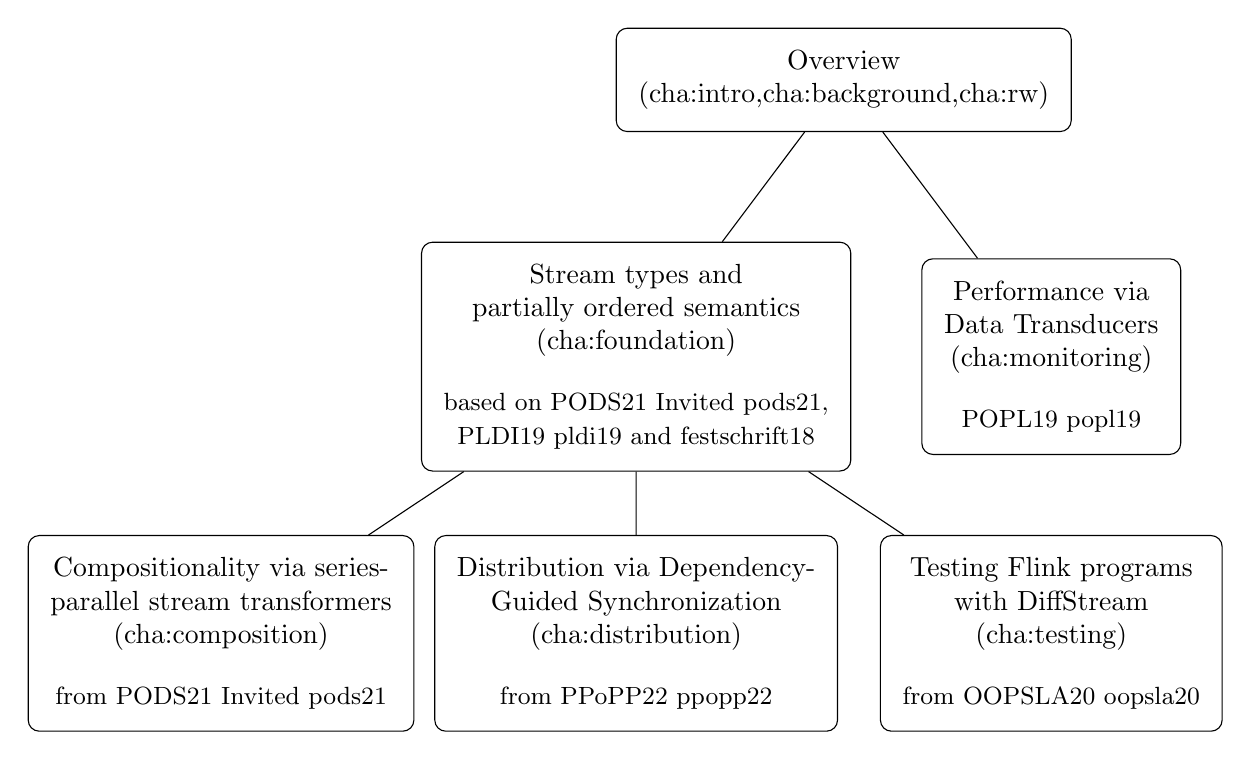
\begin{tikzpicture}[%
    sibling distance=15em,
    level distance=10em,
    every node/.style = {%
      shape=rectangle,
      rounded corners,
      inner sep=0.8em,
      draw,
      align=center
    }
  ]
  \node {
    Overview \\
    (\Cref{cha:intro,cha:background,cha:rw})
  }
    child {
      node {
        Stream types and \\
        partially ordered semantics \\
        (\Cref{cha:foundation}) \\[1em]
        \small based on PODS21 Invited~\citeMain{pods21}, \\
        \small PLDI19~\citeMain{pldi19} and~\citeMain{festschrift18}
      }
      child {
        node {
          Compositionality via series-\\
          parallel stream transformers \\
          (\Cref{cha:composition}) \\[1em]
          \small from PODS21 Invited~\citeMain{pods21}
        }
      }
      child {
        node {
          Distribution via Dependency-\\
          Guided Synchronization \\
          (\Cref{cha:distribution}) \\[1em]
          \small from PPoPP22~\citeMain{ppopp22}
        }
      }
      child {
        node {
          Testing Flink programs \\
          with DiffStream \\
          (\Cref{cha:testing}) \\[1em]
          \small from OOPSLA20~\citeMain{oopsla20}
        }
      }
    }
    child {
      node {
        Performance via \\
        Data Transducers \\
        (\Cref{cha:monitoring}) \\[1em]
        \small POPL19~\citeMain{popl19}
      }
    }
    ;
\end{tikzpicture}

\caption{Overview of the work included in this thesis.}
\label{chapter-overview}
\end{figure}

The structure of the thesis is displayed visually in \Cref{chapter-overview}.
In summary, our contributions are as follows:

\begin{itemize}
\item
We propose a foundational type system for distributed streams based on partially ordered sets.
We show that under our type system, streams can be equivalently viewed as
structured hierarchical data called \emph{batches},
as finite sequences of events called \emph{linearizations},
or as labeled partially ordered sets (traditionally known as pomsets).
In the historical notes, we also discuss how these closely relate to
our earlier synchronization schemas~\citeMain{pods21} and data-trace types~\citeMain{pldi19}.
(\Cref{cha:foundation})

\item
We show how stream operators can be defined compositionally on top of our core type system.~\citeMain{pods21} (\Cref{cha:composition})

\item
We propose \emph{dependency-guided synchronization},
a programming model and system for safe (deterministic and semantics-preserving) distribution~\citeMain{ppopp22}.
(\Cref{cha:distribution})

\item
To detect bugs due to nondeterminism in existing DSPS applications,
we propose \emph{DiffStream}, a differential testing tool~\citeMain{oopsla20}.
In particular, we leverage the partial order viewpoint to specify
ordering requirements, and we test for violations at runtime.
(\Cref{cha:testing})

\item
Towards streaming applications with predictable performance,
we propose \emph{data transducers}, a monitoring formalism and state-machine based intermediate representation~\citeMain{popl19}.
Our formalism is compositional, enabling compilation of high-level
monitoring queries with provable performance bounds.
(\Cref{cha:monitoring})
\end{itemize}

Finally, \Cref{cha:discussion}
contains limitations, unanswered questions, and concluding remarks.

\section{Software}

The work in this thesis is implemented in a number of open-source tools available on GitHub.
\begin{samepage}
\begin{itemize}
\item \githubref{https://github.com/angelhof/flumina}{Flumina} is a parallel programming model for stream processing with safe distribution, written in Erlang with experiments against Flink and Timely Dataflow.
\item \githubref{https://github.com/fniksic/diffstream}{DiffStream} is a differential testing tool for Apache Flink.
\item \githubref{https://github.com/cdstanford/data-transducers}{Data Transducers} is an intermediate representation for streaming with formal performance guarantees, written in Rust.
\end{itemize}
\end{samepage}

\section{Attribution}

Most of the work presented in this thesis was done in close collaboration with my advisor, Rajeev Alur, and other coauthors:
particularly Konstantinos Mamouras (for \Cref{cha:monitoring}) and Konstantinos Kallas and Filip Nikšić (for \Cref{cha:distribution,cha:testing}).
I wrote all the included material in \Cref{cha:intro,cha:background,cha:foundation,cha:composition,cha:discussion}, the material on the programming model in \Cref{cha:distribution}, one of the case studies and other miscellaneous sections in \Cref{cha:testing}, and almost all the material in \Cref{cha:monitoring}.
\Cref{cha:background} incorporates material from my WPE-II written report~\citeMain{wpe2} (of which I am the sole author), and \Cref{cha:rw} integrates some text from all of the papers included in the thesis.

The software repositories Flumina and DiffStream are shared projects with my collaborators, Konstantinos Kallas and Filip Nikšić.
For Flumina, I contributed the experiments and infrastructure with Timely Dataflow in Rust, the Smart Home Power Prediction case study, and documentation.
For DiffStream, I contributed the MapReduce case study and documentation.
The Data Transducers development in Rust is solely my own work.
